\part{Химическая технология}
{\bfseries МРНТИ 31.23.21}

\sectionwithauthors{О.А.Нуркенов, А.Ж.Мендибаева, Т.М.Сейлханов, Ж.С.Нурмаганбетов, С.К.Кабиева, А.К.Сыздыков, С.Д.Фазылов}{CИНТЕЗ И МОДИФИКАЦИЯ АЗИДА НИКОТИНОВОЙ КИСЛОТЫ}

\begin{center}
{\bfseries \textsuperscript{1,2}О.А.Нуркенов, \textsuperscript{1,2}А.Ж.Мендибаева, \textsuperscript{3}Т.М.Сейлханов, Ж.С.Нурмаганбетов\textsuperscript{1,4}, \textsuperscript{2}С.К.Кабиева, \textsuperscript{1,2}А.К.Сыздыков, \textsuperscript{1}С.Д.Фазылов}

\textsuperscript{1}Институт органического синтеза и углехимии,
Караганда, Казахстан,

\textsuperscript{2}Карагандинский индустриальный университет, Темиртау,
Казахстан,

\textsuperscript{3}Кокшетауский университет им. Ш. Уалиханова, Кокшетау,
Казахстан,

\textsuperscript{4}Медицинский университет Караганды, Караганда,
Казахстан

Корреспондент-автор: \emph{iosu8990@mail.ru}
\end{center}

Производные никотиновой кислоты обладают широким спектром биологической
активности и находят различное применение в медицинской практике в
качестве препаратов первой линий для лечения туберкулеза {[}1{]},
легочной артериальной гипертензии {[}2{]}, эпилепсии, зависящей от
витамина B6 {[}3{]}, ингибиторов фактора свертывания крови IXa
{[}4,5{]}, ингибиторов вируса иммунодефицита человека {[}6,7{]} и др.
Следует отметить, что пиридиновый цикл входит в состав многих жизненно
важных органических соединений, что определяет одну из его доминирующих
ролей среди гетероциклов. Поэтому разработка удобных методов синтеза
новых производных никотиновой кислоты является актуальной проблемой,
поскольку эти соединения представляют интерес как в практическом, так и
в теоретическом плане. Целью данной работы является целенаправленный
синтез азида никотиновой кислоты и осуществление его дальнейшей
модификации с целью получения новых фармакологически активных
соединений.

В настоящей работе осуществлен синтез азида никотиновой кислоты
взаимодействием нитрита натрия с гидразидом никотиновой кислоты с
выходом 99\%. Изучено взаимодействие азида никотиновой кислоты со
спиртами (изопропиловый и бутиловый спирты) и вторичным амином
(алкалоидом цитизином). Показано, что при нагревании в среде сухого
бензола азид никотиновой кислоты претерпевает перегруппировку Курциуса,
с образованием изоцианата, который далее реагирует \emph{in situ} со
спиртами и амином (алкалоидом цитизином) с образованием соответствующих
уретанов и мочевины. С целью синтеза производных 1,2,3-триазола
осуществлено взаимодействие азида никотиновой кислоты с терминальным
ацетиленом - проп-2-иниловым эфиром
3-трет-бутил-5-этил-2-гидроксибензойной кислоты в среде ДМФА и
нагревании (70-80\textsuperscript{о}С) в присутствии медного купороса
СuSO\textsubscript{4}×5H\textsubscript{2}O и аскорбата натрия (NaAsc).
Установлено, что в результате реакции образуется не ожидаемое
1,2,3-триазольное соединение, а 3-аминопиридин и исходное ацетиленовое
соединение. Показано, что при нагревании получаемый азид разлагается с
образованием промежуточной частицы - нитрена, и последующая миграция
пиридильного радикала к атому азота (перегруппировка Курциуса) приводит
к изоцианату. В результате гидратации изоцианата и последующего
декарбоксилирования из образовавшейся карбаминовой кислоты получается
3-аминопиридин. Строение синтезированных соединений подтверждено на
основании анализа данных ЯМР \textsuperscript{1}Н- и
\textsuperscript{13}С-спектроскопии, а также двумерных спектров COSY
(\textsuperscript{1}H-\textsuperscript{1}H) и HMQC
(\textsuperscript{1}H-\textsuperscript{13}C).

{\bfseries Ключевые слова}: азид никотиновой кислоты, гидразид,
перегруппировка Курциуса, изоцианат, уретан, мочевина,
ЯМР\textsuperscript{1}Н и \textsuperscript{13}С спектроскопия.

\begin{center}
{\large\bfseries НИКОТИН ҚЫШҚЫЛЫ АЗИДІНІҢ СИНТЕЗІ ЖӘНЕ МОДИФИКАЦИЯСЫ}

{\bfseries \textsuperscript{1,2}О.А.Нүркенов, \textsuperscript{1,2}Ә.Ж
Меңдібаева, \textsuperscript{3}Т.М.Сейілханов,}

{\bfseries \textsuperscript{1,4}Ж.С.Нұрмағанбетов,
\textsuperscript{2}С.Қ.Қабиева, \textsuperscript{1,2}А.Қ.Сыздықов,
\textsuperscript{1}С.Д.Фазылов}

\textsuperscript{1}Қазақстан Республикасының Органикалық синтез және
көмір химиясы институты, Қарағанды, Қазақстан,

\textsuperscript{2} Қарағанды индустриалды университеті, Теміртау,
Қазақстан,

\textsuperscript{3} Ш. Уәлиханов атындағы Көкшетау университеті,
Көкшетау, Қазақстан,

\textsuperscript{4}Қарағанды медицина университеті, Қарағанды, Қазақстан

е-mail: iosu8990@mail.ru
\end{center}

Никотин қышқылының туындылары биологиялық белсенділіктің кең спектріне
ие және медициналық тәжірибеде туберкулезді емдеуде бірінші қатардағы
препараттар ретінде {[}1{]}, өкпе артериялық гипертензиясын {[}2{]},
В\textsubscript{6} витаминіне тәуелді эпилепсияны {[}3{]}, қан ұю
факторының IXa ингибиторын {[}4,5{]}, адамның иммун тапшылығы вирусының
ингибиторын емдеуге арналған препараттар ретінде әртүрлі қолдануды
табады {[}6,7{]}. Пиридин циклі көптеген өмірлік маңызды органикалық
қосылыстардың құрамына кіретінін атап өткен жөн, бұл оның гетероциклдер
арасындағы басым рөлдердің бірін анықтайды. Сондықтан никотин қышқылының
жаңа туындыларын синтездеудің ыңғайлы дайындық әдістерін жасау өзекті
мәселе болып табылады, өйткені бұл қосылыстар практикалық және теориялық
қызығушылық тудырады. Бұл жұмыстың мақсаты - никотин қышқылы азидінің
мақсатты синтезі және жаңа фармакологиялық белсенді қосылыстар алу үшін
оны одан әрі түрлендіру.

Бұл жұмыста никотин қышқылы азидінің синтезі 99\% шығыммен натрий
нитритінің никотин гидразидімен өзара әрекеттесуі арқылы жүзеге
асырылды. Никотин қышқылы азидінің спирттермен (изопропил және бутил
спирттері) және екіншілік аминмен (цитизин алкалоидымен) өзара
әрекеттесуі зерттелді. Құрғақ бензол ортасында қыздырылған кезде никотин
қышқылының азиді Курцийдің қайта түрленуінен өтіп, реакцияға қабілетті
өнім изоцианат түзеді, ол \emph{in situ} жағдайында спирттермен және
алкалоид цитизинмен әрекеттесіп, жаңа уретандар мен мочевина түзеді.
1,2,3-триазол туындыларын синтездеу мақсатында никотин қышқылы азидінің
ДМФА ортасында 3-трет-бутил-5-этил-2-гидроксибензой қышқылының
терминалдық ацетилен-проп-2-инил эфирімен және
СuЅО\textsubscript{4}×5H\textsubscript{2}O мыс сульфаты мен натрий
аскорбатының (NaAsc) қатысуыда қыздырумен (70-80\textsuperscript{о}С)
өзара әрекеттесуі жүзеге асырылды. Реакция нәтижесінде, күтілетін
1,2,3-триазол қосылысы емес, 3-аминопиридин және бастапқы ацетилен
қосылысы түзілетіні анықталды. Қыздырылған кезде бастапқы түзілген азид
ыдырап, аралық бөлшек - нитрен түзетіні көрсетілді, пиридил радикалының
азот атомына кейінгі миграциясы (Курцийдің қайта құрылуы) изоцианатқа
әкеледі. Изоцианаттың ылғалдануы және нәтижесінде пайда болған карбамин
қышқылының декарбоксилденуі нәтижесінде 3-аминопиридин алынады.
Синтезделген қосылыстардың құрылымы ЯМР \textsuperscript{1}Н - және
\textsuperscript{13}С-спектроскопия әдістерімен, сондай-ақ СOSY
(\textsuperscript{1}H-\textsuperscript{1}H) және HMQC
(\textsuperscript{1}H-\textsuperscript{13}C) екі өлшемді спектрлерінің
деректерімен расталды.

{\bfseries Түйін сөздер:} никотин қышқылының азиді, гидразид, Курциустің
қайта топтастыруы, изоцианат, уретан, мочевина, ЯМР \textsuperscript{1}Н
және \textsuperscript{13}С спектроскопия.

\begin{center}
{\large\bfseries SYNTHESIS AND MODIFICATION OF NICOTINIC ACID AZIDE}

{\bfseries \textsuperscript{1,2}O.A.Nurkenov,
\textsuperscript{1,2}A.Zh.Mendibayeva,
\textsuperscript{3}T.M.Seilkhanov,}

{\bfseries \textsuperscript{1,4}Zh.S.Nurmaganbetov,
\textsuperscript{2}S.K.Kabieva, \textsuperscript{1,2}A.K.Syzdykov,
\textsuperscript{1}S.D.Fazylov}

\textsuperscript{1}Institute of Organic Synthesis and Coal Chemistry,
Karaganda, Kazakhstan,

\textsuperscript{2}Karaganda Industrial University, Kazakhstan,
Temirtau, Kazakhstan,

\textsuperscript{3}Sh. Ualikhanov Kokshetau University, Kokshetau,
Kazakhstan,

\textsuperscript{4}Medical University of Karaganda, Karaganda,
Kazakhstan

е-mail: iosu8990@mail.ru
\end{center}

Nicotinic acid derivatives have a wide range of biological activity and
are widely used in medical practice as first-line drugs for the
treatment of tuberculosis {[}1{]}, pulmonary arterial hypertension
{[}2{]}, vitamin B\textsubscript{6}-dependent epilepsy {[}3{]},
inhibitors of blood clotting factor IXa {[}4, 5{]}, human
immunodeficiency virus inhibitor {[}6,7{]}, etc. It should be noted that
the pyridine cycle is part of many vital organic compounds, which
determines it's one of the dominant roles among heterocycles. Therefore,
the development of convenient preparative methods for the synthesis of
new nicotinic acid derivatives is an urgent task, since these compounds
are of practical and theoretical interest. The purpose of this work is
the targeted synthesis of nicotinic acid azide and its further
modification in order to obtain new pharmacologically active compounds.

In this work, the synthesis of nicotinic acid azide was carried out by
the interaction of sodium nitrite with nicotinic hydrazide with a yield
of 99\%. The interaction of nicotinic acid azide with alcohols
(isopropyl and butyl alcohols) and a secondary amine (cytisine alkaloid)
has been studied. It has been shown that when heated in a dry benzene
medium, nicotinic acid azide undergoes a Curcius rearrangement to form
isocyanate, which reacts \emph{in situ} with alcohols and the alkaloid
cytisine to form the corresponding urethanes and urea. In order to
synthesize 1,2,3-triazole derivatives, the interaction of nicotinic acid
azide with terminal acetylene - prop-2-inyl ether of
3-tert-butyl-5-ethyl-2-hydroxybenzoic acid was carried out in a DMFA and
heated (70-80 °C) in the presence of copper sulfate
CuSO\textsubscript{4}×5H\textsubscript{2}O and sodium ascorbate (NaAsc).
It was found that as a result of the reaction, not the expected
1,2,3-triazole compound is formed, but 3-aminopyridine and the initial
acetylene compound. It is shown that when heated, the azide decomposes
to form an intermediate particle, nitrene, and the subsequent migration
of the pyridyl radical to the nitrogen atom (Curtius rearrangement)
leads to isocyanate. As a result of hydration of isocyanate and
subsequent decarboxylation of the resulting carbamic acid,
3-aminopyridine is obtained. \emph{Conclusion.} The synthesis of
nicotinoylazide was carried out by the interaction of sodium nitrite
with nicotinic acid hydrazide. The interaction of nicotinic acid azide
with terminal acetylen - prop-2-vinyl ester of
3-tert-butyl-5-ethyl-2-hydroxybenzoic acid did not lead to the formation
of the expected 1,2,3-triazole compound. It was found that the initial
azide undergoes Curcius rearrangement upon heating \emph{in situ} with
the formation of corresponding urethanes and urea. The structure of the
synthesized compounds was confirmed by NMR \textsuperscript{1}H and
\textsuperscript{13}C spectroscopy, as well as data from the
two-dimensional spectra COZY (\textsuperscript{1}H-\textsuperscript{1}H)
and HMQC (\textsuperscript{1}H-\textsuperscript{13}C).

{\bfseries Keywords:} nicotinic acid azide, hydrazide, Curtius
rearrangement, isocyanate, urethane, urea, \textsuperscript{1}H and
\textsuperscript{13}C NMR spectroscopy.

\begin{multicols}{2}
{\bfseries Введение.} Органические азиды являются универсальными
строительными блоками для различных областей химии и являются весьма
реакционно-способными соединениями и часто используются в качестве
интермедиатов в тонком органическом синтезе. Они находят широкое
применение в биохимии в качестве защитных групп {[}8{]}, как
универсальные линкеры {[}9,10{]}, также перспективным является
использование лекарственных препаратов, в структуре которых есть азидная
группа, для лечения вирусов иммунодефицита человека и герпеса {[}11{]}.
В последнее время возрастает интерес к органическим азидам как к
перспективным реагентам для динамично развивающейся «\emph{click
chemistry}», в частности, после открытия медь-катализируемой реакции
циклоприсоединения азидов и терминальных алкинов с образованием
триазолов {[}12{]}. К сожалению, в литературе мало подробных данных о
синтезе и модификации азидов пиридинкарбоновых кислот. Тем не менее,
попытки представить информацию о методах синтеза новых производных
азидов пиридинкарбоновых кислот активности продолжаются.

{\bfseries Материалы и методы.} \emph{Экспериментальная часть.} Спектры ЯМР
\textsuperscript{1}Н и \textsuperscript{13}С снимали на спектрометре
JNM-ECA 400 (399.78 и 100.53 МГц соответственно) с использованием
растворителя ДМСО-\emph{d\textsubscript{6}}. Контроль за ходом реакции и
чистотой полученных соединений осуществляли методом тонкослойной
хроматографии на пластинках Silufol UV-254 в системах изопропиловый
спирт-бензол-аммиак (10:5:2) (проявление парами йода).

\emph{Методики синтеза азида никотиновой кислоты и его производных.}

\emph{Азид никотиновой кислоты (2).} К раствору 2,23 г (0,016 М)
гидразида никотиновой кислоты в 3,5 мл концентрированной азотной кислоты
(95\%) и 2 мл воды прибавляют при 0±2\textsuperscript{о}С по каплям
раствор 2,7 г (0,039М) нитрита натрия в 5 мл воды. Осадок белый порошок
отфильтровывают, фильтрат подщелачивают 20\%-ным раствором
Na\textsubscript{2}CO\textsubscript{3} и отфильтровывают еще
дополнительное количество азида. Общий выход 3,2 г (99 \% от теорет.),
т.пл. 47-48\textsuperscript{о}С. Спектр ЯМР \textsuperscript{1}Н
(CDCl\textsubscript{3}), δ, м.д., (\emph{J}, Гц): 7.38-7.42 м (1Н,
Н\textsuperscript{1}), 8.25-8.28 м (1Н, Н\textsuperscript{4}), 8.80-8.81
(1Н, Н\textsuperscript{2}), 8.19 с (1Н, Н\textsuperscript{6}). Спектр
ЯМР \textsuperscript{13}С (CDCl\textsubscript{3}), δ\textsubscript{С},
м.д.: 123.45 (С\textsuperscript{3}), 126.48 (С\textsuperscript{5}),
136.63 (С\textsuperscript{4}), 150.58 (С\textsuperscript{6}), 154.53
(С\textsuperscript{2}), 171.17 (С\textsuperscript{7}).

\emph{3-Аминопиридин (5).} Смесь никотиноилазида (2) (1 г, 6.751 ммоль),
замещенного ацетилена (5) (1.75 г, 6.751 ммоль),
СuSO\textsubscript{4}×5Н\textsubscript{2}О (0.084 г, 0.337 ммоль) и
аскорбата натрия (0.066 г, 0.337 ммоль) в ДМФА (8 мл) перемешивают при
75°С в течение 8-10 ч (контроль ТСХ). Выпавший при охлаждении осадок
отфильтровывают, промывают гексаном, сушат, получают 3-аминопиридин (5).
Для выделения 3-аминопиридина (5) растворитель отгоняют в вакууме,
остаток хроматографируют на колонке с силикагелем (элюент - хлороформ,
смесь хлороформа с этанолом, 100:1 → 10:1). После колоночной
хроматографии выделяют 0,74 г (42\%) 3-аминопиридин (5) с т. пл.
175-180\textsuperscript{о}С и непрореагировавшее исходное ацетиленовое
соединение (3). Спектр ЯМР \textsuperscript{1}Н (CDCl\textsubscript{3} +
CD\textsubscript{3}OD), δ, м.д., (\emph{J}, Гц): 6.30 с (2Н,
Н\textsuperscript{7,7}), 7.44-7.46 м (1Н, Н\textsuperscript{3}),
7.70-7.72 м (1Н, Н\textsuperscript{4}), 8.44-8.46 (1Н,
Н\textsuperscript{2}), 8.71 с (1Н, Н\textsuperscript{6}). Спектр ЯМР
\textsuperscript{13}С (CDCl\textsubscript{3}), δ\textsubscript{С}, м.д.:
122.00 (С\textsuperscript{4}), 124.80 (С\textsuperscript{3}), 137.85
(С\textsuperscript{6}), 139.00 (С\textsuperscript{2}), 146.20
(С\textsuperscript{5}).

\emph{Изопропил-пиридин-3-ил карбомат (6).} К 0,5 г (0,0033 М)
никотиноилазиду (2) в 10 мл бензоле добавляют при перемешивании 0,26 г
(0,0043 М) изопропилового спирта. Реакционную смесь кипятят в течение 1
часа, а затем охлаждают до комнатной температуры. Сырой продукт
отфильтровывают, сушат и перекристаллизовают этилацетатом. Выход
продукта составляют 0,3 г (44,11 \%), светло-желтый порошок, т.пл.
138-140\textsuperscript{о}С. ИК спектр (KBr), ν, см\textsuperscript{-1}:
3415 (NH), 1685 (CO\textsubscript{амид}). Спектр ЯМР
\textsuperscript{1}Н (CDCl\textsubscript{3}), δ, м.д., (\emph{J}, Гц):
1.28 с (6Н, Н\textsuperscript{11,11,11,13,13,13}), 4.97-5.03 м (1Н,
Н\textsuperscript{10}), 8.66 с (1Н, Н\textsuperscript{7}), 7.21-7.24 м
(Н, Н\textsuperscript{3}), 8.27-8.28 м (1Н, Н\textsuperscript{2}), 8.03
с (1Н, Н\textsuperscript{4}), 8.50 с (1Н, Н\textsuperscript{6}). Спектр
ЯМР \textsuperscript{13}С (CDCl\textsubscript{3}), δ\textsubscript{С},
м.д.: 22.32 (С\textsuperscript{11,13}), 69.24 (С\textsuperscript{10}),
153.60 (С\textsuperscript{8}), 123.87 (С\textsuperscript{3}), 125.98
(С\textsuperscript{4}), 135.72 (С\textsuperscript{5}), 140.13
(С\textsuperscript{6}), 143.95 (С\textsuperscript{2}). Спектр ЯМР COSY:
Н\textsuperscript{11,13}→Н\textsuperscript{10},
Н\textsuperscript{3}→Н\textsuperscript{2}. Спектр ЯМР HMQC:
Н\textsuperscript{11,13}→С\textsuperscript{11,13},
Н\textsuperscript{10}→С\textsuperscript{10},
Н\textsuperscript{3}→С\textsuperscript{3},
H\textsuperscript{4}→С\textsuperscript{4},
Н\textsuperscript{2}→С\textsuperscript{2},
H\textsuperscript{6}→С\textsuperscript{6}. Спектр ЯМР HMBC:
Н\textsuperscript{11,13}→С\textsuperscript{10};
Н\textsuperscript{3}→С\textsuperscript{5};
Н\textsuperscript{4}→С\textsuperscript{2};
Н\textsuperscript{2}→С\textsuperscript{3};
Н\textsuperscript{6}→С\textsuperscript{4}, С\textsuperscript{5},
С\textsuperscript{2}.

\emph{Бутил-пиридин-3-ил карбомат (7).} К никотиноилазиду 0,5 г (0,0033
М) в 10 мл бензоле добавляют при перемешивании 0,32 г (0,0043 М)
бутанола. Реакционную смесь кипятят в течение 1 часа, а затем охлаждают
до комнатной температуры. Сырой продукт отфильтровывают и сушат. Выход
продукта составляет 0,47 г (64\%), белый порошок, т. пл.
72-75\textsuperscript{о}С. Спектр ЯМР \textsuperscript{1}Н
(CDCl\textsubscript{3}), δ, м.д., (\emph{J}, Гц): 0.88-0.93 м (3Н,
Н\textsuperscript{13,13,13}), 1.33-1.40 м (2Н,
Н\textsuperscript{12,12}), 1.60-1.67 м (2Н, Н\textsuperscript{11,11}),
4.15-4.18 м (2Н, Н\textsuperscript{10,10}), 8.58 уш. с (1Н,
Н\textsuperscript{7}), 7.23-7.26 м (1Н, Н\textsuperscript{3}), 8.28-8.29
м (1Н, Н\textsuperscript{2}), 8.10 с (1Н, Н\textsuperscript{4}), 8.52 с
(1Н, Н\textsuperscript{6}). Спектр ЯМР \textsuperscript{13}С
(CDCl\textsubscript{3}), δ\textsubscript{С}, м.д.: 13.81
(С\textsuperscript{13}), 19.14 (С\textsuperscript{12}), 31.16
(С\textsuperscript{11}), 65.46 (С\textsuperscript{10}), 123.97
(С\textsuperscript{3}), 126.00 (С\textsuperscript{4}), 135.93
(С\textsuperscript{5}), 139.88 (С\textsuperscript{6}), 143.77
(С\textsuperscript{2}), 154.26 (С\textsuperscript{8}). Спектр ЯМР COSY:
Н\textsuperscript{13}→Н\textsuperscript{12},
Н\textsuperscript{12}→Н\textsuperscript{11},
Н\textsuperscript{11}→Н\textsuperscript{10},
Н\textsuperscript{3}→Н\textsuperscript{2}. Спектр ЯМР HMQC:
Н\textsuperscript{13}→С\textsuperscript{13},
H\textsuperscript{12}→С\textsuperscript{12},
Н\textsuperscript{11}→С\textsuperscript{11},
Н\textsuperscript{10}→С\textsuperscript{10},
Н\textsuperscript{3}→С\textsuperscript{3},
H\textsuperscript{4}→С\textsuperscript{4},
Н\textsuperscript{2}→С\textsuperscript{2},
H\textsuperscript{6}→С\textsuperscript{6}. Спектр ЯМР HMBC:
Н\textsuperscript{13}→С\textsuperscript{12}, С\textsuperscript{11};
Н\textsuperscript{12}→С\textsuperscript{13}, С\textsuperscript{11},
С\textsuperscript{10}; Н\textsuperscript{11}→С\textsuperscript{13},
С\textsuperscript{12}, С\textsuperscript{10};
Н\textsuperscript{10}→С\textsuperscript{12}, С\textsuperscript{11},
С\textsuperscript{8}; Н\textsuperscript{3}→С\textsuperscript{5},
С\textsuperscript{2}; Н\textsuperscript{4}→С\textsuperscript{2};
Н\textsuperscript{2}→С\textsuperscript{4};
Н\textsuperscript{6}→С\textsuperscript{4}, С\textsuperscript{5},
С\textsuperscript{2}.

\emph{N'-(Пиридин-3-ил)цитизино-карбоксиамид (8).} К цитизину 0,5129 г
(0,0026 М) в 11,7 мл воде добавляют при перемешивании 0,108 г (0,0026 М)
натрия гидроксида. Прибавляют 0,5 г (0,0033 М) никотиноилазида
поддерживая рН=9,0-10,0 при помощи карбоната калия. Реакционную смесь
перемешивают в течение 2 ч. Сырой продукт отфильтровывают и сушат,
остаток хроматографировывают на колонке с силикагелем (элюент -
хлороформ, смесь хлороформа с этанолом, 100:1 → 10:1). Выход продукта
0,4 г (41 \%), густое масло. ИК спектр (KBr), ν, см\textsuperscript{-1}:
3462 (NH), 1647 (CO\textsubscript{амид}). Спектр ЯМР
\textsuperscript{1}Н (CDCl\textsubscript{3}), δ, м.д., (\emph{J}, Гц):
1.99 с (2Н, Н\textsuperscript{13ax,14)}, 2.41-2.52 м (1Н,
Н\textsuperscript{13eq}), 2.83-3.31 м (3Н,
Н\textsuperscript{11ax,11eq,12}), 3.62-3.82 (2Н, м,
Н\textsuperscript{15ax,22ax}), 4.01-4.20 м (1H,
Н\textsuperscript{15eq}), 4.79 уш. с (1Н, Н\textsuperscript{22eq}),
5.81-5.94 м (1Н, Н\textsuperscript{20}), 6.35-6.46 м (1Н,
Н\textsuperscript{18}), 7.15-7.24 м (4Н, Н\textsuperscript{19,3,4,6}),
8.02 с (1Н, Н\textsuperscript{7}), 8.50 с (1Н, Н\textsuperscript{2}).
Спектр ЯМР \textsuperscript{13}С (CDCl\textsubscript{3}),
δ\textsubscript{С}, м.д.: 26.24 (С\textsuperscript{14}), 27.89
(С\textsuperscript{13}), 34.88 (С\textsuperscript{12}), 48.60 и 48.69
(С\textsuperscript{15} и С\textsuperscript{22}), 54.95
(С\textsuperscript{11}), 105.41 (С\textsuperscript{20}), 117.96
(С\textsuperscript{18}), 123.38 (С\textsuperscript{3},
С\textsuperscript{4}), 131.16 (С\textsuperscript{5}), 134.75
(С\textsuperscript{6}), 147.38 (С\textsuperscript{21}), 148.93
(С\textsuperscript{19}), 150.76 (С\textsuperscript{2}), 163.30
(С\textsuperscript{8}), 168.66 (С\textsuperscript{17}). Спектр ЯМР COSY:
Н\textsuperscript{14}→Н\textsuperscript{13ax},
Н\textsuperscript{13ax}→Н\textsuperscript{12},
Н\textsuperscript{20}→Н\textsuperscript{19},
Н\textsuperscript{18}→Н\textsuperscript{19}. Спектр ЯМР HMQC:
Н\textsuperscript{13ax,13eq,14}→С\textsuperscript{13,14},
H\textsuperscript{12}→С\textsuperscript{12},
Н\textsuperscript{11ax}→С\textsuperscript{11},
Н\textsuperscript{15eq}→С\textsuperscript{15},
Н\textsuperscript{15ax,22ax}→С\textsuperscript{15,22},
H\textsuperscript{20}→С\textsuperscript{20},
Н\textsuperscript{18}→С\textsuperscript{18},
H\textsuperscript{3}→С\textsuperscript{3},
H\textsuperscript{19}→С\textsuperscript{19},
H\textsuperscript{2}→С\textsuperscript{2}. Спектр ЯМР HMBC:
Н\textsuperscript{14}→С\textsuperscript{13},
Н\textsuperscript{14}→С\textsuperscript{12},
Н\textsuperscript{14}→С\textsuperscript{15,22},
Н\textsuperscript{14}→С\textsuperscript{11},
Н\textsuperscript{14}→С\textsuperscript{21}.

{\bfseries Результаты и обсуждение.} Нами в течение ряда лет проводятся
исследования по синтезу и изучению фармакологических свойств новых
производных никотиновой кислоты {[}13-17{]}. В настоящей работе, в целях
расширения арсенала биоактивных веществ производных никотиновой кислоты,
осуществлен синтез азида и проведена его дальнейшая модификация. Синтез
азида никотиновой кислоты осуществлялась действием водного раствора
нитрита натрия на гидразид никотиновой кислот {\bfseries (1)} в смеси
концентрированной соляной кислоты и воды при охлаждении реакционной
смеси (0±2\textsuperscript{о}С). В результате реакций с количественным
выходом (99\%) получен азид никотиновой кислоты {\bfseries (2)}.
\end{multicols}

\begin{figure}[H]
	\centering
	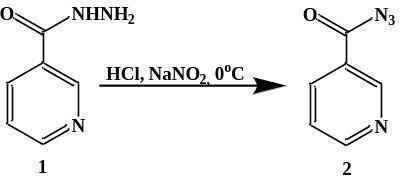
\includegraphics[width=0.5\textwidth]{assets/1}
\end{figure}

Строение соединения {\bfseries 2} было подтверждены методами ИК-, ЯМР
\textsuperscript{1}Н- и \textsuperscript{13}С-спектроскопии.

В ИК-спектре азида {\bfseries 2} имеются полосы поглощения азидной и
амидной групп: в области 2136 и 1263 см\textsuperscript{-1} присутствуют
полосы поглощения, характер-ные для N=N группы азидного фрагмента, а
полоса поглощения амидной группы C(O)NH проявляется в области 1687
см\textsuperscript{-1} (рисунок 1).

Спектр ЯМР \textsuperscript{1}Н соединения -- азида никотиновой кислоты
{\bfseries (2)} пиридиновые протоны Н-3, Н-4 и Н-2 проявились
однопротонными мультиплетами при 7.38-7.42, 8.25-8.28 и 8.80-8.81 м.д.
Пиридиновый протон Н-6 регистрировался однопротонным синглетом при 8.19
м.д.

\begin{figure}[H]
	\centering
	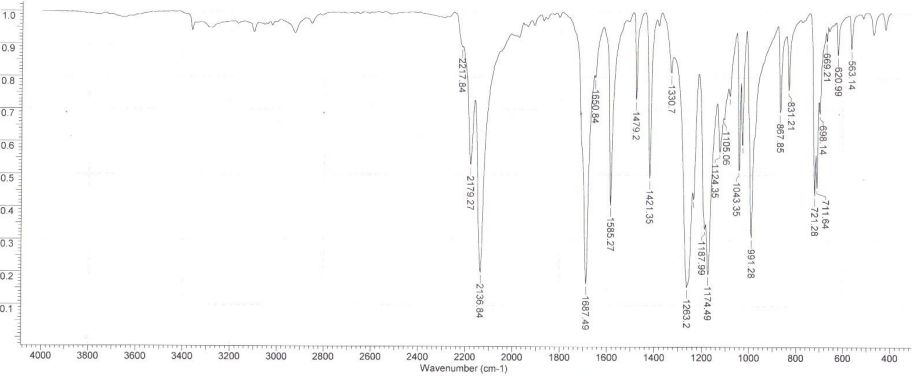
\includegraphics[width=\textwidth]{assets/2}
	\caption*{Рис.1 -- ИК спектр азида никотиновой кислоты (2) (КBr)}
\end{figure}

В спектре ЯМР \textsuperscript{13}С соединения {\bfseries 2} сигналы
углеродных атомов пиридинового фрагмента проявились при 123.45 (С-3),
126.48 (С-5), 136.63 (С-4), 150.58 (С-6) и 154.53 (С-2) м.д. Атомы
углерода карбонильной группы С-7 проявились при 171.17 м.д.

Для оценки реакционной способности азида никотиновой кислоты {\bfseries 2}
были проведены реакции взаимодействия азида {\bfseries 2} со спиртами и
вторичным амином. Реакции образования производных 1,2,3-триазола путём
конденсации органических азидов с алкинами в присутствии Cu(I)
(циклоприсоединение Хьюсгена) {[}12{]} была выбрана как возможный способ
получения мультифункциональных соединений («двойных лекарств») на основе
азида никотиновой кислоты. Учитывая тот факт, что азид никотиновой
кислоты образуется с хорошим выходом в достаточно мягких условиях, нами
было сделано предположение, что реакция с различными алкинами, в
присутствии соединений Cu(I) в качестве катализатора, могут привести к
замещённым производным, содержащим фрагмент 1,2,3-триазола.

В результате проведенных исследований установлено, что взаимодействие
никотиноилазида {\bfseries (2)} с терминальным ацетиленом спиртом -
проп-2-иниловым эфиром 3-трет-бутил-5-этил-2-гидроксибензойной кислоты
{\bfseries (3)} в среде ДМФА и нагревании (70-80\textsuperscript{о}С) в
присутствии медного купороса СuSO\textsubscript{4}×5H\textsubscript{2}O
в присутствии аскорбата натрия (NaAsc) не приводит к образованию
ожидаемого 1,2,3-триазольного соединения {\bfseries 4}. После очистки
реакционной массы на Флеш колонке полученный новый продукт был
охарактеризован как 3-аминопиридин {\bfseries (5)} с выходом 42\% и
исходное ацетиленовое соединение {\bfseries 3}.

Строение выделенных продуктов {\bfseries 3} и {\bfseries 5} было доказано
методами ЯМР\textsuperscript{1}Н-, \textsuperscript{13}С- спектроскопии.
Так, в спектре ЯМР \textsuperscript{1}Н соединения {\bfseries 5}
пиридиновые протоны Н-3, Н-4 и Н-2 проявились однопротонными
мультиплетами при 7.44-7.46, 7.70-7.72 и 8.44-8.46 м.д. Пиридиновый
протон Н-6 регистрировался однопротонным синглетом при 8.71 м.д. Аминные
протоны Н-7,7 проявились двухпротонным синглетом при 6.30 м.д.

\begin{figure}[H]
	\centering
	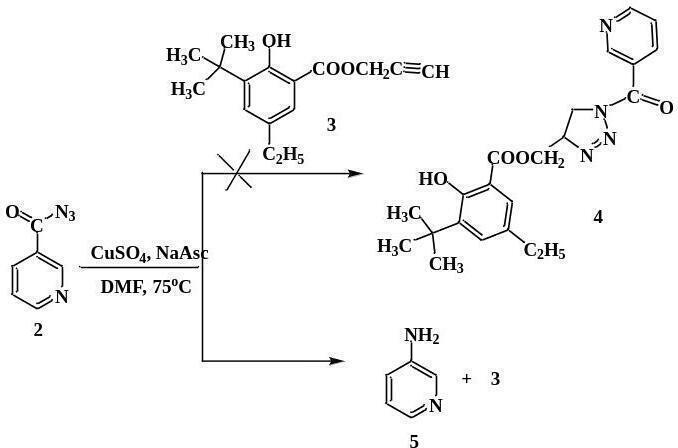
\includegraphics[width=0.8\textwidth]{assets/3}
	\caption*{}
\end{figure}

В спектре ЯМР \textsuperscript{13}С соединения {\bfseries 5} сигналы
углеродных атомов пиридинового фрагмента проявились при 122.00 (С-4),
124.80 (С-3), 137.85 (С-6), 139.00 (С-2) и 146.20 (С-5) м.д.

В спектре ЯМР \textsuperscript{1}Н ацетиленового соединения {\bfseries 3}
метильные протоны Н-11,11,11 проявились трехпротонным мультиплетом при
1.17-1.21 м.д. Метильные протоны Н-9,9,9,14,14,14,15,15,15
регистрировались трехпротонным синглетом при 1.38 м.д. Метиленовые
протоны Н-10,10 проявились двухпротонным мультиплетом при 2.51-2.54 м.д.
Ацетиленовый протон Н-19 регистрировался однопротонным синглетом при
2.58 м.д. Метиленовые протоны Н-17,17 проявились двухпротонным
мультиплетом при 4.91-4.92 м.д. Ароматические протоны Н-3 и Н-5
регистрировались однопротонными синглетами при 7.29 и 7.56 м.д.
соответственно. Гидроксильный протон Н-7 резонировал однопротонным
синглетом при 11.09 м.д.

Показано, что при нагревании азид {\bfseries 2} разлагается с образованием
промежуточной частицы ({\bfseries I}) --- нитрена, последующая миграция
пиридильного радикала к атому азота (перегруппировка Курциуса) приводит
к изоцианату ({\bfseries II}). В результате гидратации изоцианата
{\bfseries II} и последующего декарбоксилирования образовавшейся
карбаминовой кислоты ({\bfseries III}) получается 3-аминопиридин
{\bfseries (5)}.

\begin{figure}[H]
	\centering
	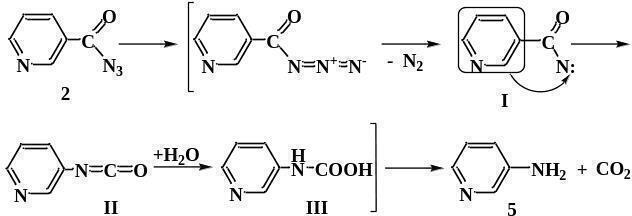
\includegraphics[width=0.8\textwidth]{assets/4}
	\caption*{}
\end{figure}

Результаты проведенных исследований по синтезу 1,2,3-триазолсодержащего
производного на основе азида никотиновой кислоты не привели к желаемому
целевому продукту {\bfseries 4} - конечными продуктами были 3-аминопиридин
{\bfseries 5} и исходное ацетиленовое соединение {\bfseries 3}.

Продолжая наши исследования в области синтеза биологически активных
веществ, мы рассмотрели возможность использования перегруппировки
Курциуса при превращении азида никотиновой кислоты в изоцианат с
последующим его взаимодействием с соединениями, несущими активный атом
водорода, такими как спирты, амины и т.д., которые обычно приводят к
образованию уретанов, мочевин и других соединений {[}16{]}.

В научной литературе для синтеза изоцианата широко используется
перегруппировка, включающее образование ацил- и арилнитренов как общих
интермедиатов {[}17{]}. Эти перегруппировки происходят за счет наличия
электронного секстета у атома азота. При перегруппировке по Курциусу
азида ароматической кислоты распадается при нагревании на изоцианат с
выделением азота.

В связи с этим мы провели взаимодействие никотиноилазида со спиртами
(изопропиловый и бутиловый спирты). Поскольку изоцианат легко образуется
при нагревании азида никотиновой кислоты в безводной среде {[}17{]},
отпадает необходимость его предварительного выделения. При нагревании в
среде сухого инертного растворителя (бензол) азид никотиновой кислоты
{\bfseries (2)} претерпевает перегруппировку Курциуса, с образованием
изоцианата, который реагирует \emph{in situ} со спиртами при кипячении в
течение 1-2 часов с образованием соответствующих уретанов {\bfseries 6},
{\bfseries 7}, выделяемых в твердом виде из реакционной среды.

\begin{figure}[H]
	\centering
	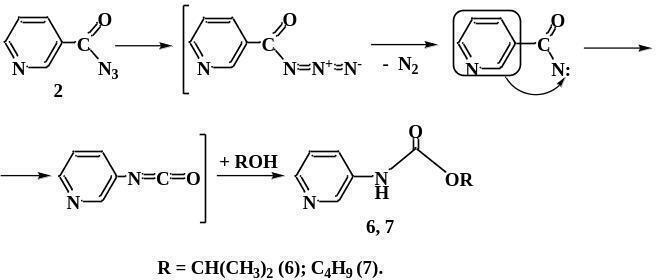
\includegraphics[width=0.8\textwidth]{assets/5}
	\caption*{}
\end{figure}

Строение синтезированных уретанов {\bfseries 6}, {\bfseries 7} доказаны
методами ЯМР\textsuperscript{1}Н-, \textsuperscript{13}С- и двумерной
спектроскопии HMQC (\textsuperscript{1}H-\textsuperscript{13}C),
позволяющей установить спин-спиновые взаимодействия протонов с атомами
углерода гетероядерной природы. Так, спектр ЯМР \textsuperscript{1}Н
соединения {\bfseries 7} характеризуется присутствием четырех мультиплетных
сигналов бутилкарбаматного фрагмента при 0.88-0.93 (3Н, Н-13, 13, 13),
1.33-1.40 (2Н, Н-12, 12), 1.60-1.67 (2Н, Н-11, 11) и 4.15-4.18 (2Н,
Н-10, 10) м.д. Карбаматный протон Н-7 проявился уширенным синглетом с
наложением на пиридиновые протоны при 8.58 м.д. Пиридиновые протоны
проявились однопротонными мультиплетами при 7.23-7.26 (Н-3) и 8.28-8.29
(Н-2) и однопротонными синглетами при 8.10 (Н-4) и 8.52 (Н-6) м.д.

\begin{figure}[H]
	\centering
	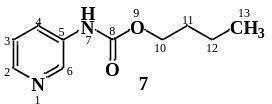
\includegraphics[width=0.8\textwidth]{assets/6}
	\caption*{}
\end{figure}

В спектре ЯМР \textsuperscript{13}С соединения {\bfseries 7} сигналы
углеродных атомов бутилкарбаматного фрагмента проявились при 13.81
(С-13), 19.14 (С-12), 31.16 (С-11), 65.46 (С-10) и 154.26 (С-8) м.д.
Углеродные атомы пиридинового фрагмента регистрировались при 123.97
(С-3), 126.00 (С-4), 135.93 (С-5), 139.88 (С-6) и 143.77 (С-2) м.д.

Строение соединения {\bfseries 7} было подтверждено также методами
двумерной спектроскопии ЯМР COSY
(\textsuperscript{1}H-\textsuperscript{1}H), HMQC
(\textsuperscript{1}H-\textsuperscript{13}C) и HMВC
(\textsuperscript{1}H-\textsuperscript{13}C), позволяющей установить
спин-спиновые взаимодействия гомо- и гетероядерной природы. Наблюдаемые
корреляции ЯМР COSY (\textsuperscript{1}H-\textsuperscript{1}H) и HMQC
(\textsuperscript{1}H-\textsuperscript{13}C) в молекуле представлены на
рисунке 2.

\begin{figure}[H]
	\centering
	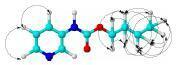
\includegraphics[width=0.8\textwidth]{assets/7}
	\caption*{}
\end{figure}a

\begin{figure}[H]
	\centering
	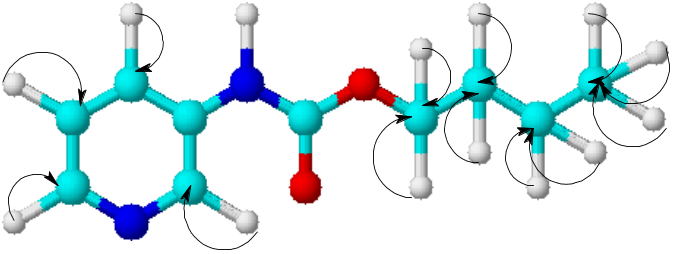
\includegraphics[width=0.8\textwidth]{assets/8}
	\caption*{}
\end{figure}b

\begin{figure}[H]
	\centering
	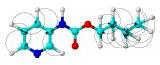
\includegraphics[width=0.8\textwidth]{assets/9}
	\caption*{}
\end{figure}c

{\bfseries Рис. 2 - Схема корреляций в спектрах COSY (а), HMQC (b) и HMBC
(с) соединения 7}

В спектрах \textsuperscript{1}H-\textsuperscript{1}H COSY соединения
{\bfseries 7} наблюдаются спин-спиновые корреляции через три связи протонов
соседних метил-метиленовых, метилен-метиленовых и метин-метинных групп
Н\textsuperscript{13}-Н\textsuperscript{12} (0.89, 1.37 и 1.37, 0.89),
Н\textsuperscript{12}-Н\textsuperscript{11e} (1.35, 1.60 и 1.60, 1.35),
Н\textsuperscript{11}-Н\textsuperscript{10} (1.60, 4.14 и 4.14, 1.60),
Н\textsuperscript{3}-Н\textsuperscript{2} (7.22, 8.26 и 8.26, 7.22) м.д.

Гетероядерные взаимодейстия протонов с атомами углерода через одну связь
были установлены с помощью спектроскопии
\textsuperscript{1}H-\textsuperscript{13}C HMQC для следующих
присутствующих в соединений пар:
Н\textsuperscript{13}-С\textsuperscript{13} (0.89, 14.00),
H\textsuperscript{12}-С\textsuperscript{12} (1.33, 19.20),
Н\textsuperscript{11}-С\textsuperscript{11} (1.61, 31.17),
Н\textsuperscript{10}-С\textsuperscript{10} (4.16, 65.52),
Н\textsuperscript{3}-С\textsuperscript{3} (7.24, 124.14),
H\textsuperscript{4}-С\textsuperscript{4} (8.11, 126.20),
Н\textsuperscript{2}-С\textsuperscript{2} (8.26, 144.29),
H\textsuperscript{6}-С\textsuperscript{6} (8.51, 139.94) м.д.

Гетероядерные взаимодействия протонов с атомами углерода через две и
более связи были установлены с помощью спектроскопии
\textsuperscript{1}H-\textsuperscript{13}C HMВC для следующих
присутствующих в соединении пар:
Н\textsuperscript{13}-С\textsuperscript{12} (0.89, 19.10),
Н\textsuperscript{13}-С\textsuperscript{11} (0.89, 31.20);
Н\textsuperscript{12}-С\textsuperscript{13} (1.35, 14.01),
Н\textsuperscript{12}-С\textsuperscript{11} (1.35, 30.99),
Н\textsuperscript{12}-С\textsuperscript{10} (1.35, 65.40);
Н\textsuperscript{11}-С\textsuperscript{13} (1.62, 14.01),
Н\textsuperscript{11}-С\textsuperscript{12} (1.62, 19.20),
Н\textsuperscript{11}-С\textsuperscript{10} (1.62, 65.63);
Н\textsuperscript{10}-С\textsuperscript{12} (4.14, 19.36),
Н\textsuperscript{10}-С\textsuperscript{11} (4.14, 30.99),
Н\textsuperscript{10}-С\textsuperscript{8} (4.14, 154.44);
Н\textsuperscript{3}-С\textsuperscript{5} (7.24, 135.61),
Н\textsuperscript{3}-С\textsuperscript{2} (7.24, 143.75);
Н\textsuperscript{4}-С\textsuperscript{2} (8.05, 143.75);
Н\textsuperscript{2}-С\textsuperscript{4} (8.27, 125.15);
Н\textsuperscript{6}-С\textsuperscript{4} (8.52, 126.08),
Н\textsuperscript{6}-С\textsuperscript{5} (8.52, 136.07),
Н\textsuperscript{6}-С\textsuperscript{2} (8.52, 144.44) м.д.

В целях расширения арсенала БАВ и изучение реакционной способности азида
никотиновой кислоты {\bfseries (2)} с аминами, проведено его взаимодействие
с молекулой алкалоида цитизина. Показано, что при нагревании в среде
сухого бензола азид никотиновой кислоты {\bfseries (2)} претерпевает
перегруппировку Курциуса с образованием изоцианата, который реагирует,
\emph{in situ}, с молекулой цитизина при кипячении в течение 1-2 часов с
образованием мочевины {\bfseries 8}. Для выделения мочевины {\bfseries 8}
растворитель отгоняют в вакууме, остаток хроматографировают на колонке с
силикагелем (элюент: хлороформ, смесь хлороформа с этанолом, 100:1 →
10:1).

\begin{figure}[H]
	\centering
	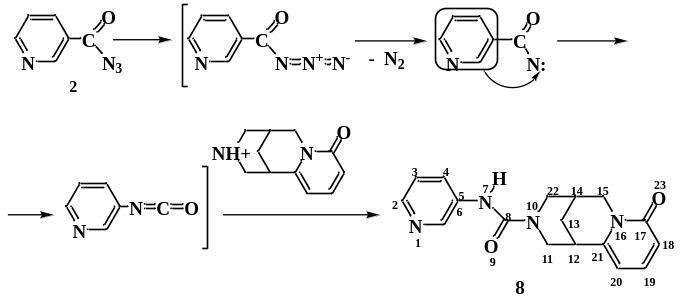
\includegraphics[width=0.8\textwidth]{assets/10}
	\caption*{}
\end{figure}

Спектр ЯМР \textsuperscript{1}Н соединения {\bfseries 8} характеризуется
присутствием сигналов протонов биспидиновых циклов цитизинового
фрагмента при 1.99 (2Н, с, Н-13ax, 14), 2.41-2.52 (1Н, м, Н-13eq),
2.83-3.31 (3Н, м, Н-11ax, 11eq, 12), 3.62-3.82 (2Н, м, 15ax, 22ax),
4.01-4.20 (1H, м, Н-15eq) и 4.79 (1Н, уш. с, Н-22eq) м.д. Ароматические
протоны цитизинового фрагмента регистрировались при 5.81-5.94 (1Н, м,
Н-20), 6.35-6.46 (1Н, м, Н-18) и при 7.15-7.24 вместе с протонами
пиридинового фрагмента (4Н, м, Н-19, 3, 4, 6) м.д. Протон Н-2
пиридинового фрагмента проявился однопротонным синглетным сигналом при
8.50 м.д. Аминный протон Н-7 регистрировался уширенным однопротонным
синглетом при 8.02 м.д.

В спектре ЯМР \textsuperscript{13}С соединения {\bfseries 8} сигналы
углеродных атомов цитизинового фрагмента молекулы проявились при 26.24
(С-14), 27.89 (С-13), 34.88 (С-12), 48.60 и 48.69 (С-15 и С-22), 54.95
(С-11), 105.41 (С-20), 117.96 (С-18), 148.93 (С-19), 147.38 (С-21),
168.66 (С-17) м.д. Углеродные атомы пиридинового фрагмента
регистрировались при 123.38 (С-3, С-4), 131.16 (С-5), 134.75 (С-6) и
150.76 (С-2) м.д. Карбамидный углеродный атом С-8 регистрировался при
1683.30 м.д.

Строение соединения {\bfseries 8} было подтверждено также методами
двумерной спектроскопии ЯМР COSY
(\textsuperscript{1}H-\textsuperscript{1}H), HMQC
(\textsuperscript{1}H-\textsuperscript{13}C) и HMВC
(\textsuperscript{1}H-\textsuperscript{13}C), позволяющей установить
спин-спиновые взаимодействия гомо- и гетероядерной природы. Наблюдаемые
корреляции ЯМР COSY (\textsuperscript{1}H-\textsuperscript{1}H) и HMQC
(\textsuperscript{1}H-\textsuperscript{13}C) в молекуле представлены на
рисунке 3.

В спектрах \textsuperscript{1}H-\textsuperscript{1}H COSY соединения
{\bfseries 8} наблюдаются спин-спиновые корреляции через три связи протонов
соседних метин-метиленовых, метилен-метиленовых и метин-метинных групп
Н\textsuperscript{14}-Н\textsuperscript{13ax} (1.85, 2.25 и 2.25, 1.85),
Н\textsuperscript{13ax}-Н\textsuperscript{12} (1.85, 2.82 и 2.82, 1.85),
Н\textsuperscript{20}-Н\textsuperscript{19} (5.91, 7.19 и 7.19, 5.91),
Н\textsuperscript{18}-Н\textsuperscript{19} (6.45, 7.23 и 7.23, 6.45)
м.д.

Гетероядерные взаимодействия протонов с атомами углерода через одну
связь были установлены с помощью спектроскопии
\textsuperscript{1}H-\textsuperscript{13}C HMQC для следующих
присутствующих в соединении пар:
Н\textsuperscript{13ax,13eq,14}-С\textsuperscript{13,14} (1.98, 26.35),
H\textsuperscript{12}-С\textsuperscript{12} (2.92, 34.59),
Н\textsuperscript{11ax}-С\textsuperscript{11} (2.95, 53.78),
Н\textsuperscript{15eq}-С\textsuperscript{15} (4.04, 49.80),
Н\textsuperscript{15ax,22ax}-С\textsuperscript{15,22} (3.73, 48.95),
H\textsuperscript{20}-С\textsuperscript{20} (5.92, 104.93),
Н\textsuperscript{18}-С\textsuperscript{18} (6.43, 117.82),
H\textsuperscript{3}-С\textsuperscript{3} (7.13, 123.10),
H\textsuperscript{19}-С\textsuperscript{19} (7.21, 139.16),
H\textsuperscript{2}-С\textsuperscript{2} (8.49, 150.99) м.д.

Гетероядерные взаимодейстия протонов с атомами углерода через две и
более связи были установлены с помощью спектроскопии
\textsuperscript{1}H-\textsuperscript{13}C HMВC для следующих
присутствующих в соединении пар:
Н\textsuperscript{14}-С\textsuperscript{13} (1.98, 27.89),
Н\textsuperscript{14}-С\textsuperscript{12} (1.98, 34.83),
Н\textsuperscript{14}-С\textsuperscript{15,22} (1.98, 48.48),
Н\textsuperscript{14}-С\textsuperscript{11} (1.98, 54.52),
Н\textsuperscript{14}-С\textsuperscript{21} (1.98, 148.52) м.д.

\begin{figure}[H]
	\centering
	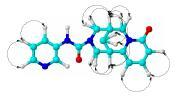
\includegraphics[width=0.8\textwidth]{assets/11}
	\caption*{}
\end{figure}a

\begin{figure}[H]
	\centering
	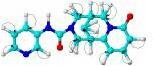
\includegraphics[width=0.8\textwidth]{assets/12}
	\caption*{}
\end{figure}b

\begin{figure}[H]
	\centering
	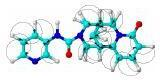
\includegraphics[width=0.8\textwidth]{assets/13}
	\caption*{}
\end{figure}c

{\bfseries Рис. 3 - Схема корреляций в спектрах COSY (а),}

{\bfseries HMQC (b) и HMBC (с) соединения 8}

Таким образом, взаимодействием азида никотиновой кислоты со спиртами
(изопропиловый и бутиловый спирты) и вторичным амином (алкалоидом
цитизин) синтезированы и охарактеризованы новые уретаны и мочевина,
строение которых подтверждены данными ЯМР \textsuperscript{1}Н- и
\textsuperscript{13}С-спектроскопии, а также анализом двумерных спектров
COSY (\textsuperscript{1}H-\textsuperscript{1}H) и HMQC
(\textsuperscript{1}H-\textsuperscript{13}C).

{\bfseries Выводы.} Осуществлен синтез никотиноилазида взаимодействием
нитрита натрия с гидразидом никотиновой кислоты. С целью синтеза
производных 1,2,3-триазола осуществлено взаимодействие азида никотиновой
кислоты с терминальным ацетиленом - проп-2-иниловым эфиром
3-трет-бутил-5-этил-2-гидроксибензойной кислоты в среде ДМФА и
нагревании (70-80\textsuperscript{о}С) в присутствии медного купороса
СuSO\textsubscript{4}×5H\textsubscript{2}O и аскорбата натрия (NaAsc).
Установлено, что в результате реакции образуется не ожидаемое
1,2,3-триазольное соединение, а 3-аминопиридин и исходное ацетиленовое
соединение. Показано, что при нагревании получаемый в ходе реакции азид
разлагается с образованием промежуточной частицы - нитрена, а
последующая миграция пиридильного радикала к атому азота
(перегруппировка Курциуса) приводит к изоцианату. В результате
гидратации изоцианата и последующего декарбоксилирования образовавшейся
карбаминовой кислоты получается 3-аминопиридин. Изучено взаимодействие
азида никотиновой кислоты со спиртами (изопропиловый и бутиловый спирты)
и вторичным амином (алкалоидом цитизином). Показано, что при нагревании
в среде сухого растворителя (бензол) азид никотиновой кислоты
претерпевает перегруппировку Курциуса с образованием изоцианата, который
реагирует \emph{in situ} со спиртами и алкалоидом цитизином с
образованием соответствующих уретанов и мочевины.

\emph{{\bfseries Финансирование}:} \emph{Научно-исследовательская работа
осуществлена в рамках ГФ АР14869941 Комитета науки Министерства науки и
высшего образования Республики Казахстан.}

{\bfseries Список литературы}

1. Timmins G.S., Master S., Rusnak F., Deretic V. Nitric oxide generated
from isoniazid activation by KATG: Source of nitric oxide and activity
against mycobacterium tuberculosis // Antimicrob. Agents Chemother.,
2004. - № 48(8).- Р. 3006-3009.

DOI 10.1128/AAC.48.8.3006-3009.2004

2. Josey J.A., Wallace E.M., Du X., Goggin B. Междунар. заявка WO
2016145032. С.А. 2016, 165, 416470.

3. Mohamed-Ahmed A.H.A., Wilson M.P., Albuera M., Chen T., Mills P.B.,
Footitt E.J., Clayton P.T., Tuleu C. Quality and stability of
extemporaneous pyridoxal phosphate preparations used in the treatment of
paediatric epilepsy //J. Pharm. Pharmacol., 2017. - № 69(4).- Р.
480-488.

DOI 10.1111/jphp.12701

4. Sakurada I., Endo Matsumoto S., Mizuno, Nosaka Y, Kato V., Maeda Y.,
Matsumoto S., Mizuno T., Nagasue H., Takeuchi K., Yokoyama T., Hruza A.,
Reichert P., Takihr K., Yokoyda S, T, inozaki M., Taguchi K, Zhang T.,
Wood H.B., Nakao K., Furusako S. Discovery of novel aminobenzisoxazole
derivatives as orally available factor IXa inhibitors // Bioorg. Med.
Chem. Lett., 2017. - №27(11) - Р. 2622-2628. DOI
10.1016/j.bmcl.2017.03.002

5. Sakurada I., Hirabayashi T., Maeda Y., Nagasue H.,Mizuno T., Xu J.,
Zhang T., Smith C., Parker D. Междунар. заявка WO 2015160636. C.A. 2015,
163,617864.

6. Eastman K.J., Parcella K.E., Peese K., Kad-Ow J.F., Naidu N.B.
Междунар. заявка WO 2015126765. С.А. 2015, 163, 363304.

7. Peese K., Wang Z., Kadow J.F., Sivaprakasam P., Naidu N.B. Пат.
3114129. Европ. С.А. 2017, 163, 363281.

8. Greenberg W.A., Priestley E.S., Sears P.S., Alper P.B., Rosenbohm C.,
Hendrix M., Hung S.C., Wong C.H. Design and synthesis of new
aminoglycoside antibiotics containing neamine as an optimal core
structure // J. Am. Chem. Soc.-1999. - №121(28).- Р. 6527-6541. DOI
10.1021/ja9910356

9. Hang H.C., Yu C., Pratt M.R., Bertozzi C.R. Probing
glycosyltransferase activities with the staudinger ligation // J. Am.
Chem. Soc.-2004. - №126(1).- Р. 6-7. DOI 10.1021/ja037692m

10. Liu L. H., Yan M. Perfluorophenyl azides: New Applications in
Surface Functionalization and Nanomaterial Synthesis // Acc. of Chem.
Res.-2010. - № 43(11).- P.1434-1443. DOI 10.1021/ar100066t

11. Piantadosi C., Marasco Jr.C. J., Morris-Natschke S.L., Meyer K.L.,
Gumus F., Surles J.R., Ishaq K.S., Kucera L.S. Synthesis and evaluation
of novel ether lipid nucleoside conjugates for anti-HIV-1 activity // J.
Med. Chem.-1991. - № 34(4).- P.1408-1414.

DOI 10.1021/jm00108a025

12. Huisgen R.1,3-Dipolar Cycloadditions. Past and Future // Angew.
Chem. - 196. - № 2(10). - Р. 565-598. DOI 10.1002/anie.196305651

13. Nurkenov O.A., Fazylov S.D., Shulgau Z.T., Аbdrasilov B.S.,
Khlebnikov A.I., Seilkhanov T.M., Kabieva S.K., Karipova G.Zh.
Synthesis, structure and antiradical activity of functionally
substituted hydrazides of isonicotinic acid // Eurasian Chem.Technol.
J.-2023. - № 25(2).- Р.121-128. DOI 10.18321/ectj1502.

14. Нуркенов О.А., Фазылов С.Д., Нурмаганбетов Ж.С., Сейлханов Т.М.,
Мендибаева А.Ж. Синтез и строение новых тиомочевинных производных
никотиновой кислоты с фрагментами природных алкалоидов // Известия НАН
РК. Серия химии и технологий\emph{. --} 2024. - №1(458).-С. 106-115. DOI
10.32014/2024.2518-1491.211

15. Нуркенов О.А., Мендибаева А.Ж., Фазылов С.Д., Сейлханов Т.М.,
Кабиева С.К., Сатбаева Э.М., Карипова Г.Ж., Сыздыков А.К. Cинтез
четвертичных аммониевых солей гидразонов изоникотиновой и никотиновой
кислот и их противовоспалительная активность // Химический журнал
Казахстана.-2024. - №1 (85).- С. 154-166.

DOI 10.51580/2024-1.2710-1185.15

16. Нестерова Е.Ю., Пугачева А.С., Воевудский М.В., Станкевич О.С.
Применение перегруппировки Курциуса в синтезе β-аминоникотиновой кислоты
// Вiсник ДНУ. Сер. Хiмiя. -2007. - №10(2).-С. 72-75.

17. Нестерова Е.Ю., Пугачева А.С., Воевудский М.В., Ващенко В.В. Реакция
гидразинолиза уретанов пиридинового ряда // Вопросы химии и химической
технологии.- 2011. - №5.- С. 33-39.

\begin{center}
{\bfseries References}
\end{center}

\begin{noparindent}
1. Timmins G.S., Master S., Rusnak F., Deretic V. Nitric oxide generated
from isoniazid activation by KATG: Source of nitric oxide and activity
against mycobacterium tuberculosis // Antimicrob. Agents Chemother.,
2004. - № 48(8).- Р. 3006-3009.

DOI 10.1128/AAC.48.8.3006-3009.2004

2. Josey J.A., Wallace E.M., Du X., Goggin B. Междунар. заявка WO
2016145032. С.А. 2016, 165, 416470.

3. Mohamed-Ahmed A.H.A., Wilson M.P., Albuera M., Chen T., Mills P.B.,
Footitt E.J., Clayton P.T., Tuleu C. Quality and stability of
extemporaneous pyridoxal phosphate preparations used in the treatment of
paediatric epilepsy //J. Pharm. Pharmacol., 2017. - № 69(4).- Р.
480-488.

DOI 10.1111/jphp.12701

4. Sakurada I., Endo Matsumoto S., Mizuno, Nosaka Y, Kato V., Maeda Y.,
Matsumoto S., Mizuno T., Nagasue H., Takeuchi K., Yokoyama T., Hruza A.,
Reichert P., Takihr K., Yokoyda S, T, inozaki M., Taguchi K, Zhang T.,
Wood H.B., Nakao K., Furusako S. Discovery of novel aminobenzisoxazole
derivatives as orally available factor IXa inhibitors // Bioorg. Med.
Chem. Lett., 2017. - №27(11) - Р. 2622-2628. DOI
10.1016/j.bmcl.2017.03.002

5. Sakurada I., Hirabayashi T., Maeda Y., Nagasue H.,Mizuno T., Xu J.,
Zhang T., Smith C., Parker D. Междунар. заявка WO 2015160636. C.A. 2015,
163,617864.

6. Eastman K.J., Parcella K.E., Peese K., Kad-Ow J.F., Naidu N.B.
Междунар. заявка WO 2015126765. С.А. 2015, 163, 363304.

7. Peese K., Wang Z., Kadow J.F., Sivaprakasam P., Naidu N.B. Пат.
3114129. Европ. С.А. 2017, 163, 363281.

8. Greenberg W.A., Priestley E.S., Sears P.S., Alper P.B., Rosenbohm C.,
Hendrix M., Hung S.C., Wong C.H. Design and synthesis of new
aminoglycoside antibiotics containing neamine as an optimal core
structure // J. Am. Chem. Soc.-1999. - №121(28).- Р. 6527-6541. DOI
10.1021/ja9910356

9. Hang H.C., Yu C., Pratt M.R., Bertozzi C.R. Probing
glycosyltransferase activities with the staudinger ligation // J. Am.
Chem. Soc.-2004. - №126(1).- Р. 6-7. DOI 10.1021/ja037692m

10. Liu L. H., Yan M. Perfluorophenyl azides: New Applications in
Surface Functionalization and Nanomaterial Synthesis // Acc. of Chem.
Res.-2010. - № 43(11).- P.1434-1443. DOI 10.1021/ar100066t

11. Piantadosi C., Marasco Jr.C. J., Morris-Natschke S.L., Meyer K.L.,
Gumus F., Surles J.R., Ishaq K.S., Kucera L.S. Synthesis and evaluation
of novel ether lipid nucleoside conjugates for anti-HIV-1 activity // J.
Med. Chem.-1991. - № 34(4).- P.1408-1414.

DOI 10.1021/jm00108a025

12. Huisgen R.1,3-Dipolar Cycloadditions. Past and Future // Angew.
Chem. - 196. - № 2(10). - Р. 565-598. DOI 10.1002/anie.196305651

13. Nurkenov O.A., Fazylov S.D., Shulgau Z.T., Аbdrasilov B.S.,
Khlebnikov A.I., Seilkhanov T.M., Kabieva S.K., Karipova G.Zh.
Synthesis, structure and antiradical activity of functionally
substituted hydrazides of isonicotinic acid // Eurasian Chem.Technol.
J.-2023. - № 25(2).- Р.121-128. DOI 10.18321/ectj1502.

14. Nurkenov O.A., Fazylov S.D., Nurmaganbetov Zh.S., Sejlhanov T.M.,
Mendibaeva A.Zh. Sintez i stroenie novyh tiomochevinnyh proizvodnyh
nikotinovoj kisloty s fragmentami prirodnyh alkaloidov // Izvestija NAN
RK. Serija himii i tehnologij. -- 2024. - №1(458).-S. 106-115. DOI
10.32014/2024.2518-1491.211

15. Nurkenov O.A., Mendibaeva A.Zh., Fazylov S.D., Sejlhanov T.M.,
Kabieva S.K., Satbaeva Je.M., Karipova G.Zh., Syzdykov A.K. Cintez
chetvertichnyh ammonievyh solej gidrazonov izonikotinovoj i nikotinovoj
kislot i ih protivovospalitel\textquotesingle naja
aktivnost\textquotesingle{} // Himicheskij zhurnal Kazahstana.-2024. -
№1 (85).- S. 154-166. DOI 10.51580/2024-1.2710-1185.15

16. Nesterova E.Ju., Pugacheva A.S., Voevudskij M.V., Stankevich O.S.
Primenenie peregruppirovki Kurciusa v sinteze β-aminonikotinovoj kisloty
// Visnik DNU. Ser. Himija. -2007. - №10(2). -- S. 72-75.

17. Nesterova E.Ju., Pugacheva A.S., Voevudskij M.V., Vashhenko V.V.
Reakcija gidrazinoliza uretanov piridinovogo rjada // Voprosy himii i
himicheskoj tehnologii. -2011.- №5.-S. 33-39.
\end{noparindent}

\emph{{\bfseries Сведения об авторах}}

\begin{noparindent}
Нуркенов О.А.-доктор химических наук, заведующий лабораторией синтеза
биологически активных веществ, Институт органического синтеза и
углехимии Республики Казахстан, Караганда, Казахстан, e-mail:
nurkenov\_oral@mail.ru;

Мендибаева А.Ж. - младший научный сотрудник, Институт органического
синтеза и углехимии Республики Казахстан, Караганда, Казахстан, e-mail:
anenyawa@mail.ru;

Фазылов С.Д.- (автор-корреспондент) - академик НАН РК, доктор химических
наук, главный научный сотрудник, Институт органического синтеза и
углехимии Республики Казахстан, Караганда, Казахстан, e-mail:
iosu8990@mail.ru;

Сеилханов Т.М. - кандидат химических наук, заведующий лабораторией
инженерного профиля ЯМР-спектроскопии, Кокшетауский Университет им.
Уалиханова, Кокшетау, Казахстан, e-mail: tseilkhanov@mail.ru;

Нурмаганбетов Ж.С.- кандидат химических наук, ведуший научный сотрудник,
Институт органического синтеза и углехимии Республики Казахстан,
Караганда, Казахстан, e-mail:nzhangeldy@mail.ru;

Кабиева С.К.-кандидат химических наук, заведующая кафедрой Химическая
технология и экология, Карагандинский индустриальный университет,
Казахстан, e-mail: kabieva.s@mail.ru;

Сыздыков А.К - .младший научный сотрудник, Институт органического
синтеза и углехимии Республики Казахстан, Караганда, Казахстан, e-mail:
ardak.syzdykov.96@inbox.ru
\end{noparindent}

\emph{{\bfseries Information about authors}}

\begin{noparindent}
Nurkenov О.А.-Doctor of chemical sciences, Head of laboratory Synthesis
of biologically active substances, Institute of Organic Synthesis and
Coal Chemistry of the Republic of Kazakhstan, Karaganda, Kazakhstan,
е-mail: nurkenov\_oral@mail.ru;

Mendibayeva A/Zh.-Junior researcher, Institute of Organic Synthesis and
Coal Chemistry of the Republic of Kazakhstan, Karaganda, Kazakhstan,
е-mail:anenyawa@mail.ru;

Fazylov S.D.(\emph{corresponding author}) - Academician of the National
Academy of Sciences of the Republic of Kazakhstan, Doctor of chemical
sciences, chief scientific officer, Institute of Organic Synthesis and
Coal Chemistry of the Republic of Kazakhstan, Karaganda, Kazakhstan,
е-mail: iosu8990@mail.ru;

Seilkhanov T.M. - Candidate of chemical sciences, Head of the laboratory
of engineering profile of NMR spectroscopy, Kokshetau Ualikhanov
University, Kokshetau, Kazakhstan, е-mail: tseilkhanov@mail.ru;

Nurmaganbetov Zh.S. - Candidate of chemical sciences, Leading
Researcher, Institute of Organic Synthesis and Coal Chemistry of the
Republic of Kazakhstan, Karaganda, Kazakhstan, е-mail:
nzhangeldy@mail.ru;

Kabieva S.K.-Candidate of chemical sciences, Head of department of
Chemical Technology and Ecology, Karaganda Industrial University,
Kazakhstan, е-mail: kabieva.s@mail;

Syzdykov A.K.-Junior researcher, Institute of Organic Synthesis and Coal
Chemistry of the Republic of Kazakhstan, Karaganda,
Kazakhstan,е-mail:ardak.syzdykov.96@inbox.ru;\newpage
\end{noparindent}
